\section{Applying Grad-CAM}
\nblink{nhs-chest-xray/analyze/grad-cam.ipynb}

An implementation of Grad-CAM is available in the Visual Attribution on GitHub \cite{visualattribution}. Visual Attribution is not available on PyPI We therefore copied the relevant code into our own GitHub repository. Visual Attribution is built on top of PyTorch, so the integration into our project was simple. Grad-CAM was run on the last layer before the linear (dense) output layer, which is a batch normalization layer. The output shape of a batch normalization layer that follows a convolutional layer is the same as the convolutional layer. Grad-CAM can therefore be applied on these too. We also tried running on the last real convolutional layer, with much worse results.

\begin{figure}[H]
    \centering
    \begin{subfigure}[t]{.45\textwidth}
        \centering
        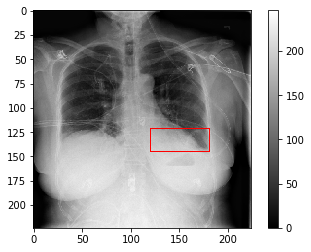
\includegraphics[width=\linewidth]{chapters/03_classification/images/rise1_bbox.png}
        \caption{Original image with bounding box added by a physician}
    \end{subfigure}\hspace{1cm}%
    \begin{subfigure}[t]{.48\textwidth}
        \centering
        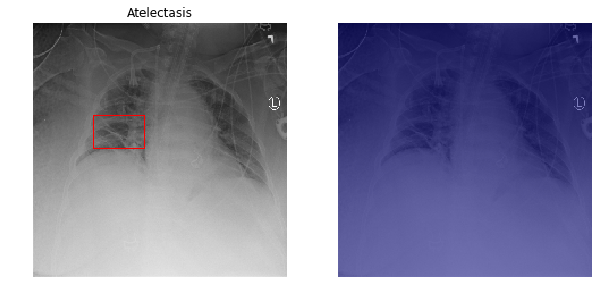
\includegraphics[width=\linewidth]{chapters/03_classification/images/grad-cam_0.png}
        \caption{Grad-CAM heat map showing important regions for the classification}
    \end{subfigure}
    \caption{The left image shows the input image with the bounding box added by the physician. The right image shows the output of Grad-CAM, which in this case is blank.}
\label{grad_cam_example_1}
\end{figure}

\begin{figure}[H]
    \centering
    \begin{subfigure}[t]{.45\textwidth}
        \centering
        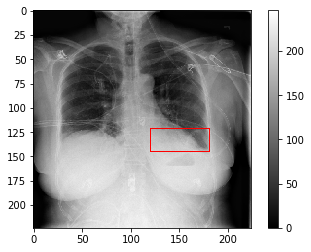
\includegraphics[width=\linewidth]{chapters/03_classification/images/rise1_bbox.png}
        \caption{Original image with bounding box added by a physician}
    \end{subfigure}\hspace{1cm}%
    \begin{subfigure}[t]{.45\textwidth}
        \centering
        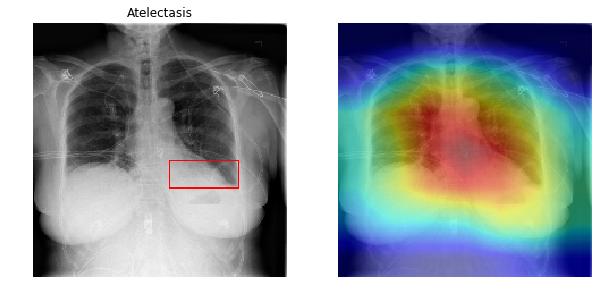
\includegraphics[width=\linewidth]{chapters/03_classification/images/grad-cam_2.png}
        \caption{Grad-CAM heat map showing important regions for the classification}
    \end{subfigure}
    \caption{The left image shows the input image with the bounding box added by the physician. The right image shows the output of Grad-CAM which contains the bounding box in the region detected as important, but the region is much bigger and its center outside of the bounding box.}
\label{grad_cam_example_2}
\end{figure}

\begin{figure}[H]
    \centering
    \begin{subfigure}[t]{.45\textwidth}
        \centering
        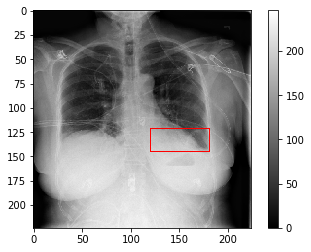
\includegraphics[width=\linewidth]{chapters/03_classification/images/rise1_bbox.png}
        \caption{Original image with bounding box added by a physician}
    \end{subfigure}\hspace{1cm}%
    \begin{subfigure}[t]{.45\textwidth}
        \centering
        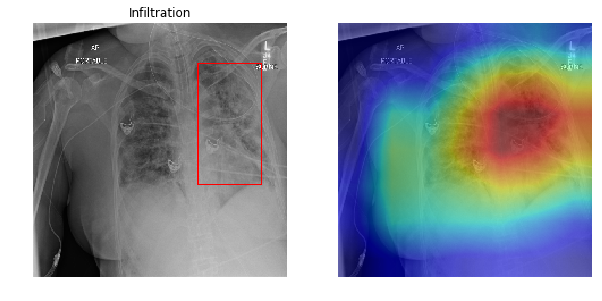
\includegraphics[width=\linewidth]{chapters/03_classification/images/grad-cam_8.png}
        \caption{Grad-CAM heat map showing important regions for the classification}
    \end{subfigure}
    \caption{The left image shows the input image with the bounding box added by the physician. The right image shows the output of Grad-CAM. The center of the output matches the bounding box.}
\label{grad_cam_example_3}
\end{figure}

\subsection{Discussion}
As seen in Figure \ref{grad_cam_example_1}, the output of Grad-CAM can be completely blank. This happens in 7 out of 21 tested images. The cause for this could not be found.

Other examples like Figure \ref{grad_cam_example_2} and Figure \ref{grad_cam_example_3} look acceptable, sometimes closely matching the bounding boxes.

\subsection{Conclusion}
The main problem with Grad-CAM is that it does not generate any output on 33\% of all images. If it actually generates output, Grad-CAM delivers usable output which most of the time marks a big part of the image as relevant for the correct classification.
